\section{유효 온도}

%(https://eesc.columbia.edu/courses/ees/slides/climate/insolation_yk.gif)

%\includegraphic[width=0.5\textwidth]{00atmospheric_science/images/insolation_yk.png}

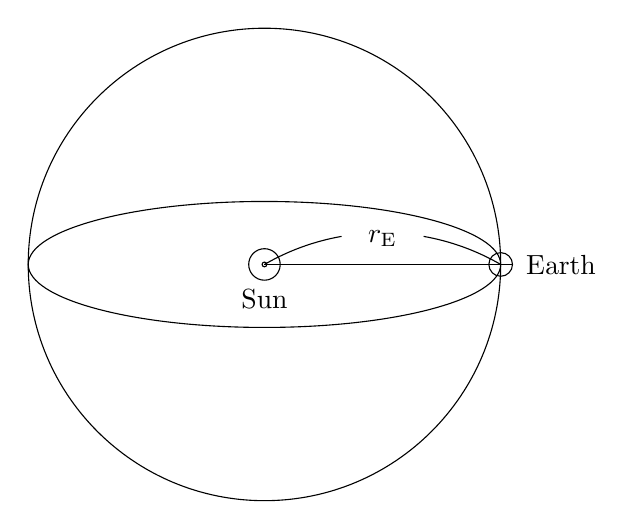
\begin{tikzpicture}
\draw (5,2) circle (3cm);
\draw (5,2) ellipse (3cm and 0.8cm);
\draw (5,2) circle (0.03cm);
\draw (5,2) circle (0.2cm) node[below, yshift=-0.2cm] {Sun};
\draw (8,2) circle (0.15cm) node[right, xshift=0.2cm] {Earth};
\draw (5,2) -- (8,2) node[above, xshift=-1.5cm, yshift=0.1cm] {$r_{\mathrm{E}}$};
\draw (5,2) arc (120:100:3cm);
\draw (8,2) arc (60:80:3cm);
\draw (7.85,2) -- (8.15,2);
\draw (8,1.85) -- (8,2.15);
\end{tikzpicture}

\begin{figure*}[h]
	\begin{tikzpicture}[rounded corners=3mm]
		\path node[rectangle,draw=green,fill=green!8,inner sep=.70cm] 
			{\parbox[t][2.5cm]{\textwidth-1.4cm-\fboxrule}
				{\question 
					* 태양의 광도($L_{\odot}$)를 이용하여 지구에서의 태양 상수($S_{\mathrm{E}}$)를 구하시오.
				\begin{solutionorlines}[2cm]
					$S_{\mathrm{E}} = \dfrac{L_{\odot}}{4\pi r_{\mathrm{E}}^{2}}$.
				\end{solutionorlines}
				}};
	\end{tikzpicture}
\end{figure*}


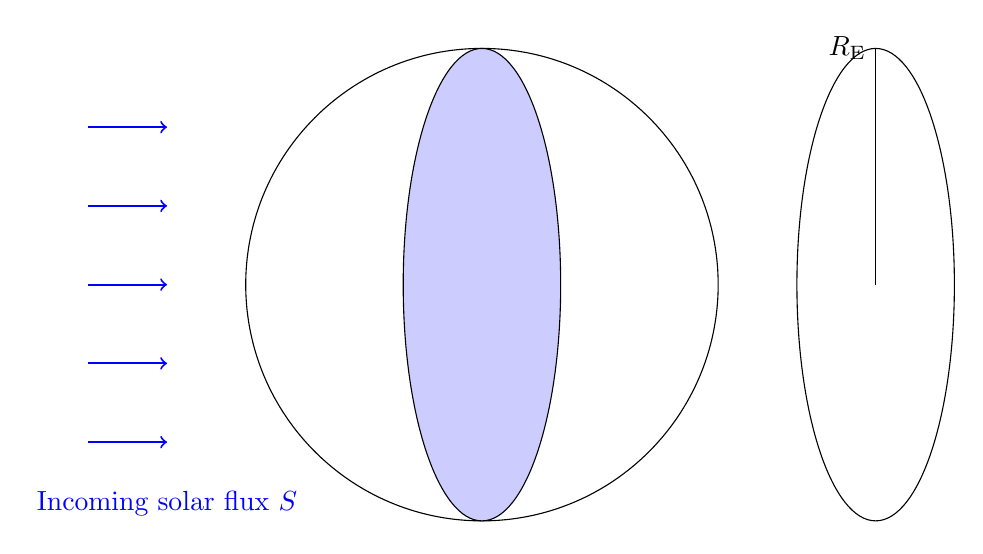
\begin{tikzpicture}
\draw [line width=0.25mm, blue] [->] (0,0) -- (1,0) node[below, yshift=-0.5cm] {Incoming solar flux $S$};
\draw [line width=0.25mm, blue] [->] (0,1) -- (1,1);
\draw [line width=0.25mm, blue] [->] (0,2) -- (1,2);
\draw [line width=0.25mm, blue] [->] (0,3) -- (1,3);
\draw [line width=0.25mm, blue] [->] (0,4) -- (1,4) ;

\draw (5,2) circle (3cm);

\fill [blue!20!white] (5,2) ellipse (1cm and 3cm) ;
\draw (5,2) ellipse (1cm and 3cm) ;
\draw (10,2) ellipse (1cm and 3cm);
\draw (10,2) -- (10,5) node[left] {$R_{\mathrm{E}}$};

\end{tikzpicture}


\begin{figure*}[h]
	\begin{tikzpicture}[rounded corners=3mm]
		\path node[rectangle,draw=green,fill=green!8,inner sep=.70cm] {\parbox[t][2.5cm]{\textwidth-1.4cm-\fboxrule}
				{\question * 지구가 받는 태양 복사 에너지 
				\begin{solutionorlines}[2cm]
					$\pi R_{\mathrm{E}}^{2} S_{\mathrm{E}}$
				\end{solutionorlines}
				}
		};
	\end{tikzpicture}
\end{figure*}




\begin{figure*}[h]
	\begin{tikzpicture}[rounded corners=3mm]
	\path node[rectangle,draw=green,fill=green!8,inner sep=.70cm] {\parbox[t][2.5cm]{\textwidth-1.4cm-\fboxrule}{
		\question * 행성에서의 태양 상수
		\begin{solutionorlines}[3cm]
			$ S_{\mathrm{P}} = S_{\mathrm{E}}\left(\dfrac{r_{\mathrm{E}}}{r_{\mathrm{P}}}\right)^{2}$
		\end{solutionorlines}
	}};
	\end{tikzpicture}
\end{figure*}


\begin{figure*}[h]
	\begin{tikzpicture}[rounded corners=3mm]
	\path node[rectangle,draw=green,fill=green!8,inner sep=.70cm] {\parbox[t][2.5cm]{\textwidth-1.4cm-\fboxrule}{
		\question 	* 행성이 받는 태양복사에너지
		\begin{solutionorlines}[2cm]
			$ \pi R_{\mathrm{P}}^{2} S_{\mathrm{E}}\left(\dfrac{r_{\mathrm{E}}}{r_{\mathrm{P}}}\right)^{2}$
		\end{solutionorlines}
	}};
	\end{tikzpicture}
\end{figure*}


\begin{questions}
	* 알베도($A$)를 고려한 행성의 행성이 받는 일사량 : 
	\begin{solution}
	$ I_{\mathrm{P}}^{\downarrow} = (1-A)\pi R_{\mathrm{P}}^{2} S_{\mathrm{E}}\left(\dfrac{r_{\mathrm{E}}}{r_{\mathrm{P}}}\right)^{2}$
	\end{solution}
\end{questions}

\begin{questions}
	* Stefan-Boltzmann 법칙 : 
	\begin{solution}
	$ I_{\mathrm{P}}^{\uparrow} = 4\pi R_{\mathrm{P}}^{2} \sigma T^{4}$
	\end{solution}
\end{questions}


\begin{questions}
	* 유효 온도 (effective temperature) : 
	\begin{solution}
	$ T_{e} = \sqrt[4]{\dfrac{(1-A) S_{\mathrm{E}}}{4 \sigma}} \sqrt{\dfrac{r_{\mathrm{E}}}{r_{\mathrm{P}}}} $
	\end{solution}
\end{questions}

유효 온도는 행성과 태양과의 거리, 알베도에 의해 결정되며 대기의 구성 성분이나 밀도 등의 물리적 성질과는 무관하다.

그러나 실제로 대기를 투과한 태양광이 대기의 구성 성분이나 지면에 흡수되고, 또 재방출 되는 복잡한 과정을 통하여 온도가 결정되므로 이러한 온도를 복사 온도(radiative temperature)라 한다. 
실제 표면 온도는 행성의 유효온도에 대기의 온실효과 등이 더해져서 결정되어진 온도이다. 
\end{questions}
%(https://solarsystem.nasa.gov/system/resources/detail_files/681_ptemp.jpg)